\section{Overview of Discrete Morphology Models} \label{sec:dm_overview}

Molecular data forms the basis of most phylogenetic analyses today. 
However, morphological characters remain relevant: Fossils often provide our only direct observation of extinct biodiversity; DNA degradation can make it difficult or impossible to obtain sufficient molecular data from fragile museum specimens. 
Using morphological data can help researchers include specimens in their phylogeny that might be left out of a molecular tree. \par
To understand how morphological characters are modeled, it is important to understand how characters are collected.
Unlike in molecular data, for which homology is algorithmically determined, homology in a character is typically assessed an expert. 
Biologists will typically decide what characters are homologous by looking across specimens at the same structure in multiple taxa; they may also look at the developmental origin of structures in making this assessment.
Once homology is determined, characters are broken down into states, or different forms a single character can take.
The state `0' commonly refers to absence, meaning that character is not present.
In some codings, absence will mean that character has not evolved in that group.
In others, absence means that that character has not evolved in that group, and/or that that character has been lost in that group. 
This type of coding is arbitrary, but both \textbf{non-random} and \textbf{meaningful}, and poses challenges for how we model the data. 
\par

Historically, most phylogenetic analyses using morphological characters have been performed using the maximum parsimony optimality criterion. 
Maximum parsimony analysis involves proposing trees from the morphological data.
Each tree is evaluated according to how many changes it implied in the data, and the tree that requires the fewest changes is preferred.
In this way of estimating a tree, a character that does not change, or changes only in one taxon, cannot be used to discriminate between trees (i.e., it does not favor a topology).
Therefore, workers with parsimony typically do not collect characters that are parsimony uninformative.
\par

In 2001, Paul Lewis introduced a generalization of the Jukes-Cantor model of sequence evolution for use with morphological data.
This model, called the Mk (Markov model, assuming each character is in one of \textit{k} states) model provided a mathemetical formulation that could be used to estimate trees from morphological data in both likelihood and Bayesian frameworks. 
While this model is a useful step forward, as a generalization of the Jukes-Cantor, it still makes fairly simplistic assumptions.
This tutorial will guide you through estimating a phylogeny with the Mk model, and two useful extensions to the model. \par

\subsection{The Mk Model}

The Mk model is a generalization of the Jukes-Cantor model of nucleotide sequence evolution, which we discussed in \textbf{Molecular Models of Character Evolution}. 
The Q matrix for a two-state Mk model looks like so:

\begin{equation*}
Q = \begin{pmatrix} -\mu_0 & \mu_{01} \\
\mu_{10} & -\mu_1  &\\
\end{pmatrix} \mbox{  ,}
\end{equation*}

This matrix can be expanded to accommodate multi-state data, as well:

\begin{equation*}
Q = \begin{pmatrix} -\mu_0 & \mu_{01} & \mu_{02} & \mu_{03} \\
\mu_{10} & -\mu_1  & \mu_{12} & \mu_{13} \\
\mu_{20} & \mu_{21} & -\mu_2  & \mu_{23} \\
\mu_{30} & \mu_{31} & \mu_{32} & -\mu_3 
\end{pmatrix} \mbox{  ,}
\end{equation*}

However, the Mk model sets transitions to be equal from any state to any other state. 
In that sense, our multistate matrix really looks like this:

\begin{equation*}
Q = \begin{pmatrix} -\mu_0 & \mu & \mu & \mu \\
\mu & -\mu_1  & \mu & \mu \\
\mu & \mu & -\mu_2  & \mu \\
\mu & \mu & \mu & -\mu_3 \\
\end{pmatrix} \mbox{  ,}
\end{equation*}

Because this is a Jukes-Cantor-like model, state frequencies do not vary as a model parameter.
These assumptions may seem unrealistic.
However, all models are a compromise between reality and generalizability.
Because morphological characters do not carry common meaning across sites in a matrix in the way that nucleotide characters do, making assumptions that fit all characters is challenging. \par

We will first perform a phylogenetic analysis using the Mk model.
In further sections, we will explore how to relax key assumptions of the Mk model. \par

\subsection{Ascertainment Bias}

When Lewis first introduced the Mk model, he observed that branch lengths on the trees were greatly inflated.
The reason for this is that when morphological characters are collected, characters that do not vary, or vary in a non-parsimony-informative way (such as autapomorphies) are excluded.
Excluding these low-rate characters causes the overall amount of evolution to be over-estimated.
This causes an inflation in the branch lengths. \par

Therefore, when performing a morphological phylogenetic analysis, it is important to correct for this bias.
Original corrections simulated invariant and non-parsimony informative characters along the proposed tree.
The likelihood of these characters would then be calculated and used to normalize the total likelihood value.
RevBayes implements a dynamic programming approach that calculates the same likelihood, but  does so faster. \par

\section{Example: Inferring a Phylogeny of Fossil Bears Using the Mk Model}

In this example, we will use morphological character data from 18 taxa of extinct bears. 
The dataset contains 62 binary characters, a fairly typical dataset size for morphological characters. \par

\medskip
\subsection{Tutorial Format}\label{subsect:Exercise-Format}

This tutorial follows a specific format for issuing instructions and information.

{\begin{framed}
The boxed instructions guide you to complete tasks that are not part of the \RevBayes syntax, but rather direct you to create directories or files or similar.
\end{framed}}


Information describing the commands and instructions will be written in paragraph-form before or after they are issued.

All command-line text, including all \Rev syntax, are given in \cl{monotype font}. 
Furthermore, blocks of \Rev code that are needed to build the model, specify the analysis, or execute the run are given in separate shaded boxes.
For example, we will instruct you to create a constant node called \cl{example} that is equal to \cl{1.0} using the \cl{<-} operator like this:
%Load the cytochrome-b sequences from file and assign the data matrix to a variable called \cl{cytb}.
{\tt \begin{snugshade*}
\begin{lstlisting}
example <- 1.0
\end{lstlisting}
\end{snugshade*}
}

It is important to be aware that some PDF viewers may render some characters given as \colorbox{shadecolor}{\tt{Rev commands}} differently. 
Thus, if you copy and paste text from this PDF, you may introduce some incorrect characters. 
Because of this, we recommend that you type the instructions in this tutorial or copy them from the scripts provided. 


\medskip
\subsection{Data and Files}\label{subsect:Exercise-DataFiles}

{\begin{framed}
On your own computer, create a directory called {\textcolor{red}{\cl{RB\_DiscreteMorphology\_Tutorial}}} (or any name you like). 

In this directory download and unzip the archive containing the data files: \href{https://github.com/revbayes/revbayes_tutorial/tree/master/RB_Discrete_Morphology_Tutorial/data.zip}{\cl{data.zip}}.

This will create a folder called \cl{data} that contains the files necessary to complete this exercise.
\end{framed}}


\bigskip
\subsection{Getting Started}\label{subsect:Exercise-GetStart}

{\begin{framed}
Create a new directory (in \cl{RB\_DiscreteMorphology\_Tutorial}) called {\textcolor{red}{\cl{scripts}}}. (If you do not have this folder, please refer to the directions in section \ref{subsect:Exercise-DataFiles}.)
\end{framed}}

When you execute \RevBayes in this exercise, you will do so within the main directory you created (\cl{RB\_DiscreteMorphology\_Tutorial}), thus, if you are using a Unix-based operating system, we recommend that you add the \RevBayes binary to your path.
\bigskip

\subsection{Creating \Rev Files}\label{subsect:Exercise-CreatingFiles}

For complex models and analyses, it is best to create \Rev script files that will contain all of the model parameters, moves, and functions. 
In this exercise, you will work primarily in your text editor\footnote{In section \ref{subsub:Req-Software} we offer a recommendation for a text editor.} and create a set of modular files that will be easily managed and interchanged.
In this first section, you will write the following files from scratch and save them in the \cl{scripts} directory:
\begin{itemize}[noitemsep,topsep=0pt]
\item \cl{mcmc\_mk.Rev}: the master \Rev file that loads the data, the separate model files, and specifies the monitors and MCMC sampler.
\item \cl{model\_mk.Rev}: specifies the model describing discrete morphological character change (binary characters). 
\end{itemize}

All of the files that you will create are also provided in the \RevBayes tutorial repository\footnote{\url{https://github.com/revbayes/revbayes_tutorial/tree/master/RB_Discrete_Morphology_Tutorial/scripts}}. 
Please refer to these files to verify or troubleshoot your own scripts. 
%TODO add link to scripts

{\begin{framed}
Open your text editor and create the master \Rev file called {\textcolor{red}{\cl{mcmc\_Mk.Rev}}} in the \cl{scripts} directory.

Enter the \Rev code provided in this section in the new model file.
\end{framed}}

The file you will begin in this section will be the one you load into \RevBayes when you've completed all of the components of the analysis.
In this section you will begin the file and write the \Rev commands for loading in the taxon list and managing the data matrices.
Then, starting in section \ref{subsect:Exercise-MkModel}, you will move on to writing module files for each of the model components. 
Once the model files are complete, you will return to editing \cl{mcmc\_Mk.Rev} and complete the \Rev script with the instructions given in section \ref{subsect:Exercise-CompleteMCMC}.

\medskip
\subsubsection{Load Data Matrices}\label{subsub:Exercise-LoadData}

\RevBayes uses the function \cl{readDiscreteCharacterData()} to load a data matrix to the workspace from a formatted file. 
This function can be used for both molecular sequences and discrete morphological characters.
Import the morphological character matrix and assign it to the variable \cl{morpho}. 
{\tt \begin{snugshade*}
\begin{lstlisting}
morpho <- readDiscreteCharacterData("data/bears.nex")
\end{lstlisting}
\end{snugshade*}}

 \medskip
\subsubsection{Create Helper Variables}\label{subsub:Exercise-mviVar}

Before we begin writing the \Rev scripts for each of the model components, we need to instantiate a couple ``helper variables'' that will be used by downstream parts of our model specification files. 
These variables will be used in more than one of the module files so it's best to initialize them in the master file.

Create a new constant node called \cl{n\_taxa} that is equal to the number of species in our analysis (18). 
We will also create a constant node of the taxon names.
This list will be used to initialize the tree.

{\tt \begin{snugshade*}
\begin{lstlisting}
taxa <- morpho.names()
n_taxa <- morpho.size() 
\end{lstlisting}
\end{snugshade*}}

Next, create a workspace variable called \cl{mvi}. 
This variable is an iterator that will build a vector containing all of the MCMC moves used to propose new states for every stochastic node in the model graph. 
Each time a new move is added to the vector, \cl{mvi} will be incremented by a value of \cl{1}.
{\tt \begin{snugshade*}
\begin{lstlisting}
mvi = 1
\end{lstlisting}
\end{snugshade*}}
One important distinction here is that \cl{mvi} is part of the \RevBayes workspace and not the hierarchical model. 
Thus, we use the workspace assignment operator \cl{=} instead of the constant node assignment \cl{<-}. 

{\begin{framed}
Save your current working version of \cl{mcmc\_Mk.Rev} in the \cl{scripts} directory.

We will now move on to the next \Rev file and will complete \cl{mcmc\_Mk.Rev} in section \ref{subsect:Exercise-CompleteMCMC}.
\end{framed}}


\bigskip
\subsection{The Mk Model}

{\begin{framed}
Open your text editor and create the master \Rev file called {\textcolor{red}{\cl{model\_Mk.Rev}}} in the \cl{scripts} directory.

Enter the \Rev code provided in this section in the new model file.
\end{framed}}

First, we will create a vector of moves on branch lengths. 
This should be familiar from the \cl{RB\_CTMC} tutorial:
{\tt \begin{snugshade*}
\begin{lstlisting}
nbr <- 2*names.size() - 3
for (i in 1:nbr){
    br_lens[i] ~ dnExponential(5.0)
    moves[mvi++] = mvScale(br_lens[i]) 
}
\end{lstlisting}
\end{snugshade*}}

Next, we will create a Q matrix. 
Recall that the Mk model is simply a generalization of the JC model.
Therefore, we will create a 2x2 Q matrix using \cl{fnJC}, which initializes Q-matrices with equal transition probabilities between all states.

{\tt \begin{snugshade*}
\begin{lstlisting}
Q_morpho := fnJC(2)
\end{lstlisting}
\end{snugshade*}}

Now that we have the basics of the model specified, we will add Gamma-distributed rate variation and specify moves on the parameter to the Gamma distribution.


{\tt \begin{snugshade*}
\begin{lstlisting}
alpha_morpho ~ dnExponential( 1.0 )
rates_morpho := fnDiscretizeGamma( alpha_morpho, alpha_morpho, 4 )

#Moves on the parameters to the Gamma distribution.
moves[mvi++] = mvScale(alpha_morpho, lambda=0.01, weight=1.0)
moves[mvi++] = mvScale(alpha_morpho, lambda=0.1,  weight=1.0)
moves[mvi++] = mvScale(alpha_morpho, lambda=1,    weight=1.0)
\end{lstlisting}
\end{snugshade*}}

Next we assemble the tree and specify a move on the topology.

{\tt \begin{snugshade*}
\begin{lstlisting}
tau ~ dnUniformTopology(names)
phylogeny := treeAssembly(tau, br_lens)
moves[mvi++] = mvSPR(tau)
\end{lstlisting}
\end{snugshade*}}

Lastly, we set up the CTMC. 
This should be familiar from the \cl{RB\_CTMC} tutorial.
We see some familiar pieces: tree, Q matrix and site\_rates.
We also have two new keywords: data type and coding.
The data type argument specifies the type of data - in our case, "Standard", the specification for morphology.
Coding specifies what type of ascertainment bias is expected.
We are using the `variable' correction, as we have no invariant character in our matrix.
If we also lacked parsimony non-informative characters, we would use the coding `informative'. 

{\tt \begin{snugshade*}
\begin{lstlisting}
phyMorpho ~ dnPhyloCTMC(tree=phylogeny, siteRates=rates_morpho, Q=Q_morpho, type="Standard", coding="variable")
phyMorpho.clamp(morpho)
\end{lstlisting}
\end{snugshade*}}

All of the components of the model are now specified. \par

\subsection{Complete Master \Rev File}\label{subsect:Exercise-CompleteMCMC}

{\begin{framed}
Return to the master \Rev file you created in section \ref{subsect:Exercise-StartMasterRev} called {\textcolor{red}{\cl{mcmc\_Mk.Rev}}} in the \cl{scripts} directory.

Enter the \Rev code provided in this section in this file.
\end{framed}}

\medskip
\subsubsection{Source Model Scripts}\label{subsub:Exercise-SourceMods}

\RevBayes uses the \cl{source()} function to load commands from \Rev files into the workspace.
Use this function to load in the model scripts we have written in the text editor and saved in the \cl{scripts} directory.
{\tt \begin{snugshade*}
\begin{lstlisting}
source("scripts/model_Mk.Rev")

\end{lstlisting}
\end{snugshade*}}


\medskip
\subsubsection{Create Model Object}\label{subsub:Exercise-ModObj}

We can now create our workspace model variable with our fully specified model DAG. 
We will do this with the \cl{model()} function and provide a single node in the graph (\cl{phylogeny}).
{\tt \begin{snugshade*}
\begin{lstlisting}
mymodel = model(phylogeny)
\end{lstlisting}
\end{snugshade*}}

The object \cl{mymodel} is a wrapper around the entire model graph and allows us to pass the model to various functions that are specific to our MCMC analysis.

\medskip
\subsubsection{Specify Monitors and Output Filenames}\label{subsub:Exercise-Monitors}

The next important step for our master \Rev file is to specify the monitors and output file names.
For this, we create a vector called \cl{monitors} that will each sample and record or output our MCMC. 

First, we will specify a workspace variable to iterate over the \cl{monitors} vector.
{\tt \begin{snugshade*}
\begin{lstlisting}
mni = 1
\end{lstlisting}
\end{snugshade*}}

The first monitor we will create will monitor every named random variable in our model graph. 
This will include every stochastic and deterministic node using the \cl{mnModel} monitor.
The only parameter that is not included in the \cl{mnModel} is the tree topology. 
Therefore, the parameters in the file written by this monitor are all numerical parameters written to a tab-separated text file that can be opened by accessory programs for evaluating such parameters.
We will also name the output file for this monitor and indicate that we wish to sample our MCMC every 10 cycles.
{\tt \begin{snugshade*}
\begin{lstlisting}
monitors[mni++] = mnModel(filename="output/mk_simple.log", printgen=10)
\end{lstlisting}
\end{snugshade*}}

The \cl{mnFile} monitor writes any parameter we specify to file.
Thus, if we only cared about the branch lengths and nothing else (this is not a typical or recommended attitude for an analysis this complex) we wouldn't use the \cl{mnModel} monitor above and just use the \cl{mnFile} monitor to write a smaller and simpler output file.
Since the tree topology is not included in the \cl{mnModel} monitor (because it is not numerical), we will use \cl{mnFile} to write the tree to file by specifying our \cl{fbd\_tree} variable in the arguments.
{\tt \begin{snugshade*}
\begin{lstlisting}
monitors[mni++] = mnFile(filename="output/mk_simple.trees", printgen=10, phylogeny)
\end{lstlisting}
\end{snugshade*}}

The last monitor we will add to our analysis will print information to the screen.
Like with \cl{mnFile} we must tell \cl{mnScreen} which parameters we'd like to see updated on the screen. 
{\tt \begin{snugshade*}
\begin{lstlisting}
monitors[mni++] = mnScreen(printgen=10)
\end{lstlisting}
\end{snugshade*}}

\medskip
\subsubsection{Set-Up the MCMC}

Once we have set up our model, moves, and monitors, we can now create the workspace variable that defines our MCMC run. 
We do this using the \cl{mcmc()} function that simply takes the three main analysis components as arguments.
{\tt \begin{snugshade*}
\begin{lstlisting}
mymcmc = mcmc(mymodel, monitors, moves)\end{lstlisting}
\end{snugshade*}}

The MCMC object that we named \cl{mymcmc} has a member method called \cl{.run()}. 
This will execute our analysis and we will set the chain length to \cl{10000} cycles using the \cl{generations} option.
{\tt \begin{snugshade*}
\begin{lstlisting}
mymcmc.run(generations=100000)
\end{lstlisting}
\end{snugshade*}}

Once our Markov chain has terminated, we will want \RevBayes to close. 
Tell the program to quit using the \cl{q()} function.
{\tt \begin{snugshade*}
\begin{lstlisting}
q()
\end{lstlisting}
\end{snugshade*}}

{\begin{framed}
You made it! Save all of your files.
\end{framed}}

\bigskip
\subsection{Execute the MCMC Analysis}\label{subsect:Exercise-RunMCMC}

With all the parameters specified and all analysis components in place, you are now ready to run your analysis. 
The \Rev scripts you just created will all be used by \RevBayes and loaded in the appropriate order.

{\begin{framed}
Begin by running the \RevBayes executable. In Unix systems, type the following in your terminal (if the \RevBayes binary is in your path):

\colorbox{black}{\strut\hspace{1mm}\textcolor[rgb]{0,1,1}{\cl{rb}}\hspace{0.925\textwidth}}
\end{framed}}

Provided that you started \RevBayes from the correct directory (\cl{RB\_TotalEvidenceDating\_FBD\_Tutorial}), you can then use the \cl{source()} function to feed \RevBayes your master script file (\cl{mcmc\_mk.Rev}).
{\tt \begin{snugshade*}
\begin{lstlisting}
source("scripts/mcmc_TEFBD.Rev")
\end{lstlisting}
\end{snugshade*}}

This will execute the analysis and you should see the following output (though not the exact same values):


{\tiny{\tt \begin{snugshade*}
\begin{lstlisting}
|* source("scripts/mcmc_mk.rev")
|*   Processing file "scripts/mcmc_mk.rev"
|*   Successfully read one character matrix from
|* file 'data/bears.nex'
|*   Processing file "scripts/mk_simple.rev"
|*   Processing of file "scripts/mk_simple.rev"
|* completed

|*   Running MCMC simulation
|*   This simulation runs 1 independent replicate.
|*   The simulator uses 37 different moves in a
|* random move schedule with 37 moves per iteration
|*
|* Iter        |      Posterior   |     Likelihood  
|* |          Prior   |    elapsed   |        ETA   
|*
|*
|* ---------------------------------------------------------------------------------------------------
|* 0           |       -685.779   |       -666.105   |       -19.6731   |   00:00:00   |   --:--:--   |

|* 10          |       -633.737   |       -608.951   |        -24.786   |   00:00:00   |   --:--:--   |

|* 20          |       -593.634   |       -558.797   |       -34.8368   |   00:00:00   |   00:00:00   |
|* 30          |       -578.661   |       -536.125   |       -42.5362   |   00:00:00   |   00:00:00   |
|* 40          |        -544.22   |       -514.098   |       -30.1223   |   00:00:00   |   00:00:00   |
|* 50          |       -515.505   |       -492.988   |       -22.5169   |   00:00:00   |   00:00:00   |
|* 60          |       -483.695   |       -461.347   |       -22.3479   |   00:00:00   |   00:00:00   |

|*...
\end{lstlisting}
\end{snugshade*}}}

When the analysis is complete, \RevBayes will quit and you will have a new directory called \cl{output} that will contain all of the files you specified with the monitors (Sect.\ \ref{subsub:Exercise-Monitors}).


\section{Example: Relaxing the Assumption of Equal Transition Probabilities }

{\begin{framed}
Make a copy of the MCMC and model files you just made. 
Call them \cl{mcmc\_mk\_dicretized.Rev} and \cl{model\_mk\_discretized.Rev}. 
These will contain the new model parameters and models. \par 
\end{framed}}

The Mk model makes a number of assumptions, but one that may strike you as unrealistic is the assumption that characters are equally likely to change from any one state to any other state.
That means that a trait is as likely to be gained as lost.
While this may hold true for some traits, we expect that it may be untrue for many others. \par
\cl{RevBayes} has functionality to allow us to relax this assumption.
We do this by specifying a Beta prior on state frequencies.
Remember from the \cl{RB\_CTMC} lesson that stationary frequencies impact how likely we are to see changes in a character.
For example, it may be very likely, in a character, to change from 0 to 1.
But if the frequency of 0 is very low, we will still seldom see this change. \par
We can exploit the relationship between state frequencies and observed changes to allow for variable Q matrices across characters.
To do this, we generate a Beta distribution on state frequencies, and use the state frequencies from that Beta distribution to generate a series of Q-matrices to use to evaluate our data. \par

\subsection{Modifying the MCMC File}

At each place in which the output files are specified in the MCMC file, change the output path so you don't overwrite the output from the previous exercise. 
For example, you might call your output file \cl{output/mk\_discretized.log} and \cl{output/mk\_discretized.trees}.
Change source statement to indicate the new model file.

\subsection{Modifying the Model File}

Open the new model file that you created. We need to modify the way in which the Q matrix is specified. 
We will use a discretized Beta distribution to place a prior on state frequencies. 
The Beta distribution has two parameters, $\alpha$ and $\beta$.
These two parameters specify the shape of the distribution.
State frequencies will be evaluated according to this distribution, in the same way that rate variation is evaluated according to the Gamma distribution. 
The discretized distribution is split into multiple classes, each with it's own set of frequencies for the 0 and 1 characters.
The number of classes can vary; we have chosen 4 for tractability.\par

{\tt \begin{snugshade*}
\begin{lstlisting}
n_cats = 4
alpha\_ofbeta ~ dnExponential( 1 )
beta\_ofbeta ~ dnExponential( 1 )
moves[mvi++] = mvScale(alpha\_ofbeta, lambda=1,    weight=1.0 )
moves[mvi++] = mvScale(alpha\_ofbeta, lambda=0.1,  weight=1.0 )
moves[mvi++] = mvScale(alpha\_ofbeta, lambda=0.01, weight=1.0 )
moves[mvi++] = mvScale(beta\_ofbeta, lambda=1,    weight=1.0 )
moves[mvi++] = mvScale(beta\_ofbeta, lambda=0.1,  weight=1.0 )
moves[mvi++] = mvScale(beta\_ofbeta, lambda=0.01, weight=1.0 )
\end{lstlisting}
\end{snugshade*}}

Above, we initialized the number of categories,  the parameters to the Beta distribution, and the moves on the parameters to the Beta. 

Next, we set the categories to each represent a quadrant of the Beta distribution specified by the \cl{alpha\_ofbeta} and \cl{beta\_ofbeta}.

{\tt \begin{snugshade*}
\begin{lstlisting}
cats := fnDiscretizeBeta(alpha_ofbeta, beta_ofbeta,4)
\end{lstlisting}
\end{snugshade*}}

If you were to print the \cl{cats} variable, you would see a list of state frequencies like so:

{\tiny{\tt \begin{snugshade*}
\begin{lstlisting}
|*   0.0780943
|*   0.40457
|*   0.769453
|*   0.97106
\end{lstlisting}
\end{snugshade*}}}

Using these state frequencies, we will generate a new vector of Q matrices.
Because we are varying the state frequencies, we must use a Q matrix generation function that allows for state frequencies to vary as a parameter.
We will, therefore, use the \cl{freeBinary} function.

{\tt \begin{snugshade*}
\begin{lstlisting}
for (i in 1:cats.size())
{
Q[i] := fnFreeBinary(v(1-cats[i], cats[i]), false)
}
\end{lstlisting}
\end{snugshade*}}

Once we've made the our vector of matrices, we specified moves on our matrix vector:
{\tt \begin{snugshade*}
\begin{lstlisting}
matrix_probs ~ dnDirichlet(v(1,1,1,1))
moves[mvi++] = mvSimplexElementScale(matrix_probs, alpha=10, weight=1.0) 
\end{lstlisting}
\end{snugshade*}}

This Dirichlet prior says that no category is expected to have more characters than another. If you expected some category to hold more of the characters, you could put more weight on that category. \par

The only other specification that needs to change in the model file is the CTMC:
{\tt \begin{snugshade*}
\begin{lstlisting}
phyMorpho ~ dnPhyloCTMC(tree=phylogeny, siteRates=rates_morpho, Q=Q, type="Standard", coding="variable", siteMatrices=matrix_probs)
\end{lstlisting}
\end{snugshade*}}

You'll notice that we've added a command to tell the CTMC that we have multiple site matrices that will be applied to different characters in the matrix.

\medskip
\subsubsection{Set-Up the MCMC}

The MCMC chain set-up does not need to change. 
Run the new MCMC file, just as you ran the plain Mk file.
This estimation will take longer than the Mk model, due to increased model complexity. \par


\section{Site-Heterogeneous Discrete Morphology Model}


In the previous example, we explored allowing among-character variation in state frequencies.
This is an excellent start for allowing more complex models for morphology.
But this approach also has several shortcomings.
First, because we use a Beta distribution, this model really only works for binary data.
Secondly, oftentimes, we will not have a good idea of the shape of the distribution from which we expect state frequencies to be drawn. \par
To accommodate for these concerns, \cl{RevBayes} also has a model that is similar to the CAT model. \par
The site-heterogeneous discrete morphology model (SHDM) uses a hyperprior on the prior on state frequencies to mix over different possible combinations state frequencies.
In this model, F81 Q-matrices (an extension of the Jukes-Cantor which allows for different state frequencies between characters) is initialized from a set of state frequencies.
The number of Q-matrices initialized is equal to the number of user-defined categories, as in the discretized Beta model.
The state frequencies used to initialize the Q-matrices are drawn from a Dirichelet prior distribution, which is generated by drawing values from an exponential hyperprior distribution. 
This model is visualized in .\par

\subsection{Example: Site-Heterogeneous Discrete Morphology Model }

{\begin{framed}
Make a copy of the MCMC and model files you just made. 
Call them \cl{mcmc\_mk\_hyperprior.Rev} and \cl{model\_mk\_hyperprior.Rev}. 
These will contain the new model parameters and models. \par 
\end{framed}}

\subsection{Modifying the MCMC File}

At each place in which the output files are specified in the MCMC file, change the output path so you don't overwrite the output from the previous exercise. 
For example, you might call your output file \cl{output/mk\_hyperprior.log} and \cl{output/mk\_hyperprior.trees}.
We will also monitor Q\_morpho and pi.
Add Q\_morpho and pi to the \cl{mnScreen}. 
Change source statement to indicate the new model file.

\subsection{Modifying the Model File}
Open the new model file that you created. We need to modify the way in which the Q-matrix is specified.
First, we will create a hyperprior called \cl{dir\_alpha} and specify a move on it.
{\tt \begin{snugshade*}
\begin{lstlisting}
dir_alpha ~ dnExponential(1)
moves[mvi++] = mvScale(dir\_alpha, lambda=1,    weight=1.0 )
moves[mvi++] = mvScale(dir\_alpha, lambda=0.1,  weight=1.0 )
moves[mvi++] = mvScale(dir\_alpha, lambda=0.01, weight=1.0 )
\end{lstlisting}
\end{snugshade*}}

This hyperparameter, dir\_alpha, will be used as a parameter to a Dirichelet distribution from which our state frequencies will be drawn.

{\tt \begin{snugshade*}
\begin{lstlisting}
pi_prior := v(dir\_alpha,dir\_alpha)
\end{lstlisting}
\end{snugshade*}}

If you were using multistate data, the dir\_alpha can be repeated for each state.
Next, we will modify our previous loop to use these state frequencies to initialize our Q-matrices.

{\tt \begin{snugshade*}
\begin{lstlisting}for(i in 1:n_cats)
{
	pi[i] ~ dnDirichlet(pi_prior)
    moves[mvi++] = mvSimplexElementScale(pi[i], alpha=10, weight=1.0) 
    
    Q_morpho[i] := fnF81(pi[i])
}
\end{lstlisting}
\end{snugshade*}}

In the above loop, for each of our categories, we make a new draw of state frequencies from our Dirichelet distribution (the shape of which is determined by our dir\_alpha values).  
We then use \cl{fnF81} to make our Q-matrices.
For each \cl{RevBayes} iteration, we will have 4 pi values and 4 Q-matrices, one for each of the number of categories we specified. \par

No other aspects of the model file need to change.
Run the MCMC as before. \par

\bigskip
\subsection{Evaluate and Summarize Your Results}\label{subsect:Exercise-SummarizeResults}

%TODO some text here
% what is interesting? What are we looking for? 

\medskip
\subsubsection{Evaluate MCMC}\label{subsub:Exercise-EvalMCMC}

In this section, we will evaluate the \textit{mixing} and \textit{convergence} of our MCMC simulation using the program {\tt Tracer}.
We can also summarize the marginal distributions for particular parameters we're interested in.
\href{http://tree.bio.ed.ac.uk/software/tracer/}{\tt Tracer} \citep{Rambaut2011} is a tool for visualizing parameters sampled by MCMC.
This program is limited to numerical parameters, however, and cannot be used to summarize or analyze MCMC samples of the tree topology (this will be discussed further in section \ref{subsub:Exercise-SummarizeTree}).

\begin{figure}[h!]
\fbox{%
\begin{minipage}{\textwidth}\centering
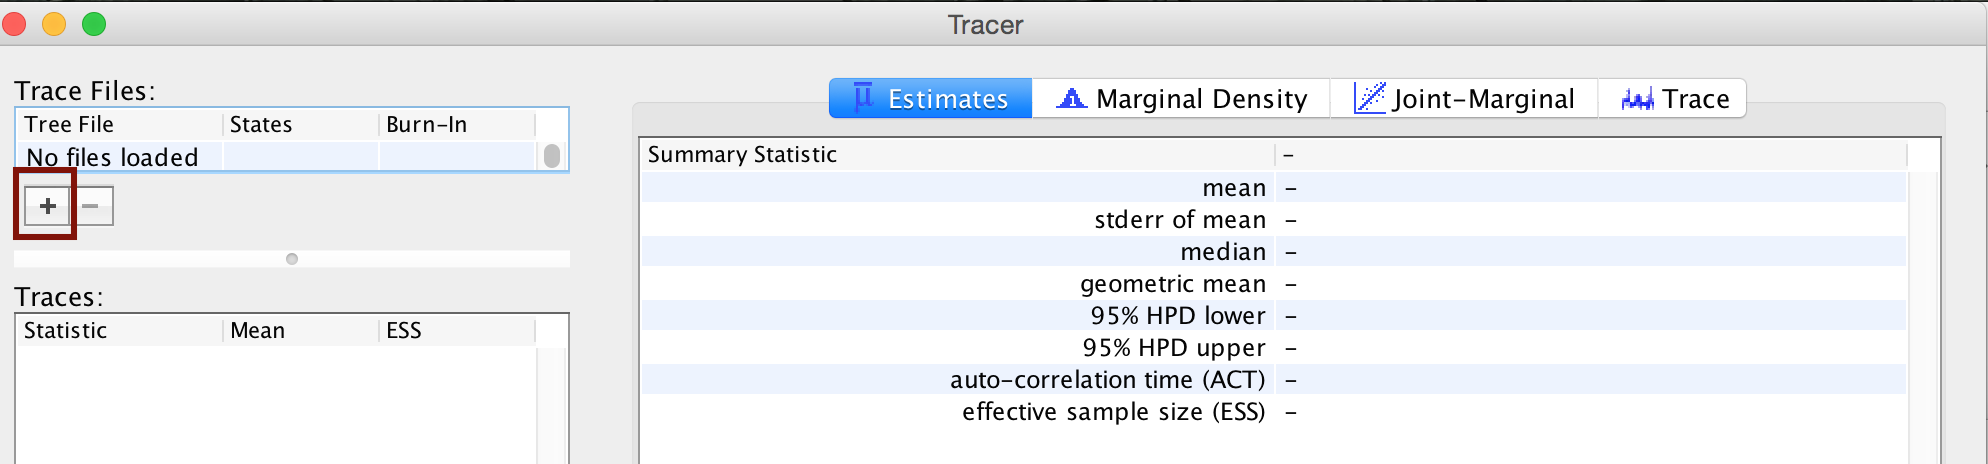
\includegraphics[width=\textwidth,angle=0]{\ResourcePath figures/tracer_load_file.png}
\caption{\small The {\tt Tracer} window. To add data, click on the ``+'' sign, highlighted in red above.}
\end{minipage}}
\label{fig:tracer}
\end{figure}


%Import the MCMC log file into Tracer.
\begin{framed}
Open {\tt Tracer} and import the log files generated by our three estimations \mi{File\textrightarrow Import New Trace File}.
Or click the \fbox{$+$} button on the left-hand side of the screen to add your log file (see Fig.\ \ref{fig:tracer}).
\end{framed}

\begin{figure}[h!]
\fbox{%
\begin{minipage}{\textwidth}\centering
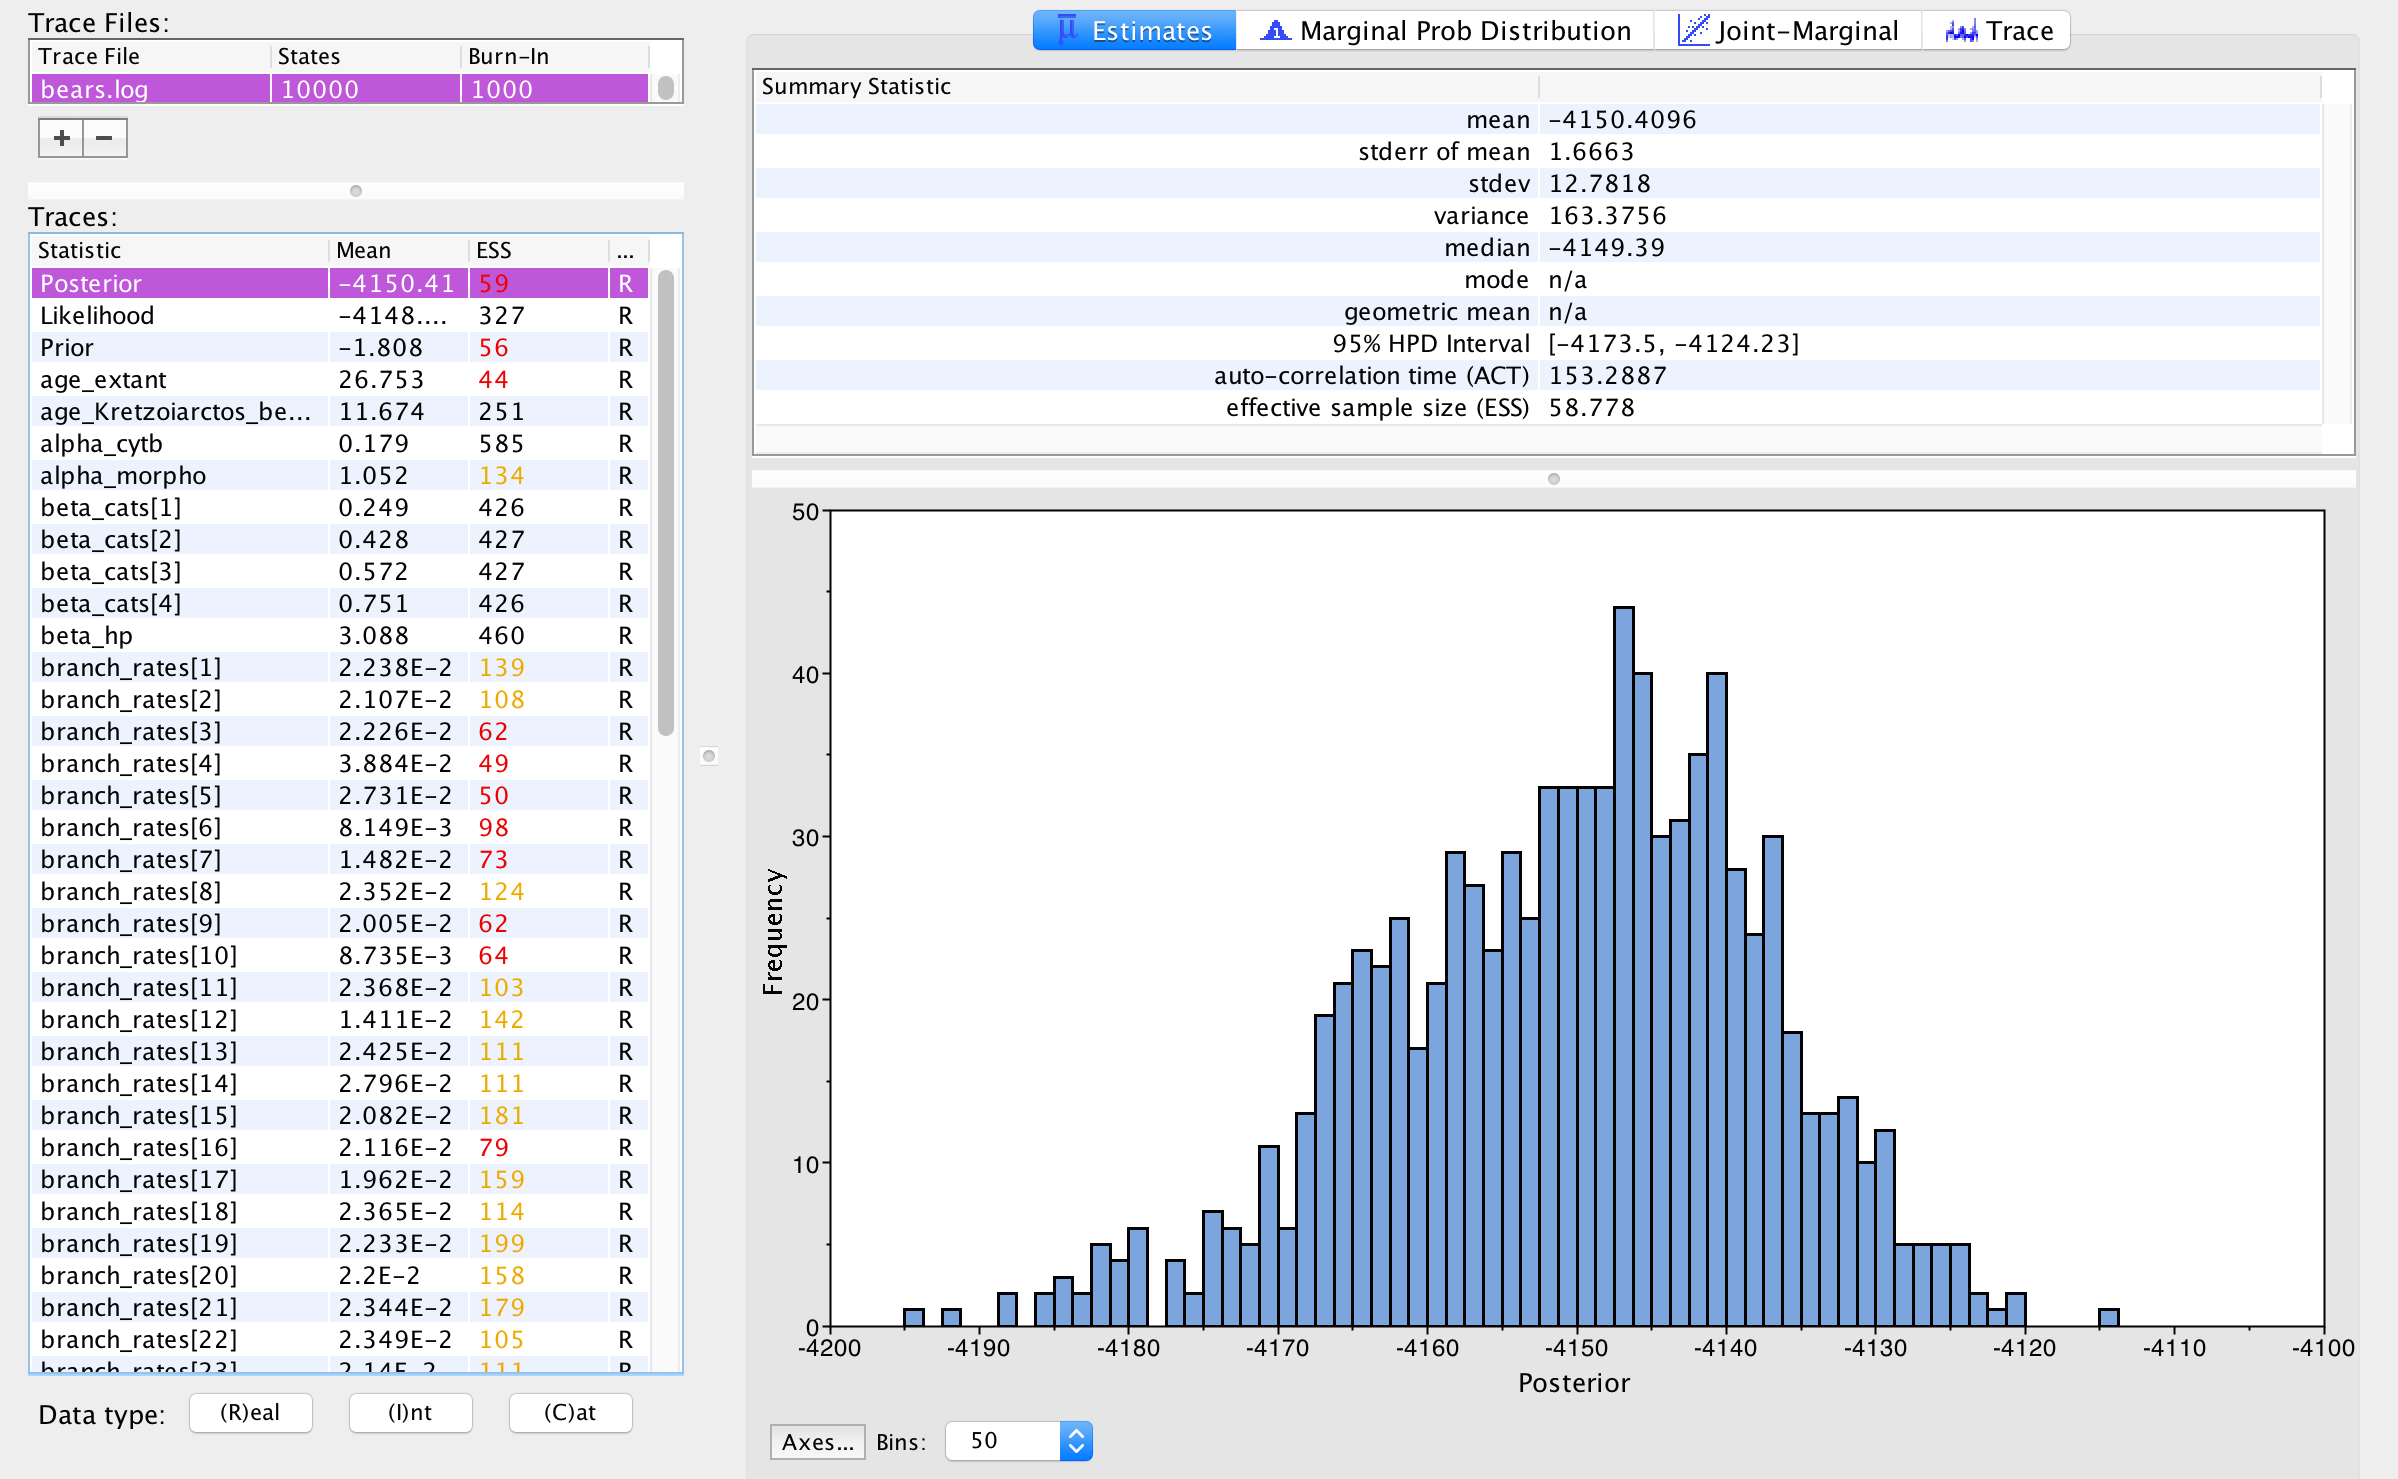
\includegraphics[width=\textwidth,angle=0]{\ResourcePath figures/tracer_fig_posterior_short.png}
\caption{\small The \mi{Estimates} window in {\tt Tracer} showing the histogram of the \mi{Posterior}.}
\end{minipage}}
\label{fig:tracer-post-ests}
\end{figure}


Immediately upon loading your file (see Fig.\ \ref{fig:tracer-post-ests}), 
you will see the list of \mi{Trace Files} on the left-hand side (you can load multiple files).
The bottom left section, called \mi{Traces}, provides a list of every parameter in the log file, along with the mean and the effective sample size (ESS) for the posterior sample of that parameter.
The ESS statistic provides a measure of the number of independent draws in our sample for a given parameter.
This quantity will typically be much smaller than the number of generations of the chain.
In {\tt Tracer}, poor to fair values for the ESS will be colored red and yellow.
You will likely see a lot of red and yellow numbers because the MCMC runs in this exercise are too short to effectively sample the posterior distributions of most parameters.
A much longer analysis is provided in the \cl{output} directory. 

The inspection window for your selected parameter is the \mi{Estimates} window, which shows a histogram and summary statistics of the values sampled by the Markov chain. 
Figure \ref{fig:tracer-post-ests} shows the marginal distribution of the \mi{Posterior} statistic for the log files in the \cl{output} directory.





\subsection{Things to consider}

...


\section{Overview of Discrete Morphology Models} \label{sec:dm_simple}

\section{Overview of Discrete Morphology Models} \label{sec:dm_complex}
{\bf \framebox{?} Alright, who did it?}

\newpage
